\section{Results}
\label{sec:results}
\subsection{Does parameterization change rotation cost after training?}
\label{sec:interaction_result}
Under the matched OpenFold Train96/ESM2-35M recipe with 1536 AdamW updates, output rotation affects the factor
head more than G+ (Figure~\ref{fig:interaction}). On Confirm96-B, the factor
contrast is \result{inter_c96_factor_rotation}, while G+'s contrast is
\result{inter_c96_gplus_rotation}. The directly estimated interaction is
\result{inter_c96_interaction}
[\result{inter_c96_interactionLo}, \result{inter_c96_interactionHi}].
The Length48 secondary comparison is also positive:
\result{inter_l48_interaction}
[\result{inter_l48_interactionLo}, \result{inter_l48_interactionHi}].
These are differences-in-differences on a 0--1 score scale, not relative
percentage improvements. The completed OpenFold Train384 four-cell controls do not
establish the interaction with either ESM2 or ESMC
(Appendix Table~\ref{tab:interaction_scope}); the positive finding is recipe-specific.

On both observed panels, all seed and rotation marginals are positive, but only
8/9 and 7/9 individual seed-by-rotation cells are positive, respectively.
On Confirm96-B, the residue-average lDDT interaction is
\result{inter_c96_interaction_residue}
[\result{inter_c96_interaction_residueLo}, \result{inter_c96_interaction_residueHi}],
and the TM-score interaction is \result{inter_c96_interaction_tm}
[\result{inter_c96_interaction_tmLo}, \result{inter_c96_interaction_tmHi}].
These metrics score the same structures, not independent samples.

G+'s direction intervals include zero on both panels, without establishing
equivalence of trained systems.

\begin{figure}[t]
\centering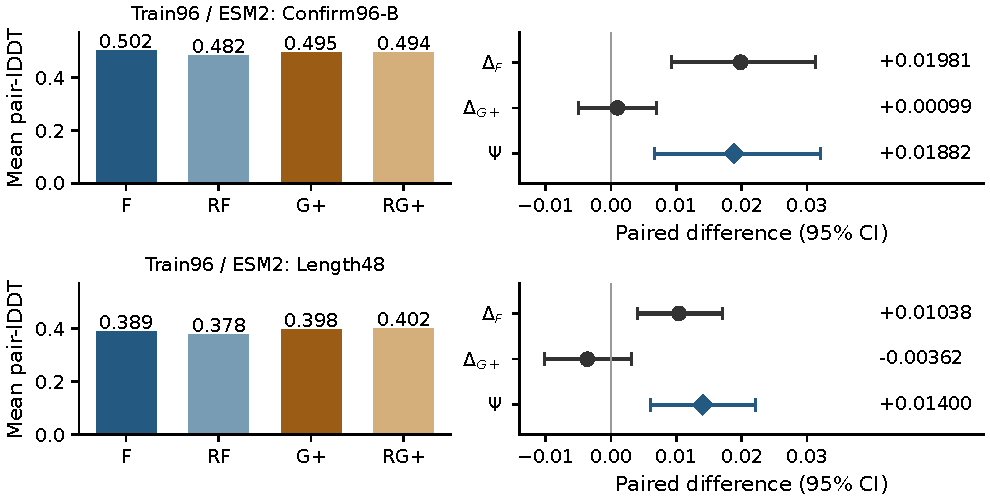
\includegraphics[width=\linewidth]{figures/interaction.pdf}
\caption{Head competitiveness and orientation sensitivity. Left: Protenix
four-cell means. Right: target-level $\Psi_i$, averaging seeds and rotations
within each panel's 48, 96 or 192 targets. Violins span observed extrema (bandwidth 0.35, equal width);
the separate, narrower axis shows $\Psi$ and its original conditional 95\% bootstrap
interval. Shaded diamonds mark the new-target primary tests: Fresh96's interval
includes zero; Fresh192's is positive. Other rows reuse observed panels and are not independent
replications (Table~\ref{tab:study_roles}). A66 multiplicity and backend limits
are in Appendix~\ref{app:dh_fourcells}.}
\label{fig:interaction}
\end{figure}

The completed Train96/Full follow-up adds three G+ and nine rotated-G+ fits,
matching the training/development manifests and 1536-update budget of the
OpenFold comparison, with Protenix's own fixed recipe. On Confirm96-B,
$\Delta_F=\result{p96_pair_factor_rotation}$ and
$\Delta_{G+}=\result{p96_pair_gplus_rotation}$ give
$\Psi=\result{p96_pair_interaction}$
[\result{p96_pair_interactionLo}, \result{p96_pair_interactionHi}].
All three seed and rotation marginals are positive; 61/96 target interactions
are positive. This extends observed-panel interaction support to a second
predictor, without providing a new-target confirmation.

The Train384 feature study completes both ESM2 and ESMC four cells
(Table~\ref{tab:coverage}; Appendix Table~\ref{tab:interaction_scope}). Its prespecified
Confirm96-B ESMC Factor contrast is \result{dh_protenix_c96_c_pair_factor_rotation}
[\result{dh_protenix_c96_c_pair_factor_rotationLo}, \result{dh_protenix_c96_c_pair_factor_rotationHi}].
The follow-up $\Psi$ is \result{dh_protenix_c96_c_pair_interaction}
[\result{dh_protenix_c96_c_pair_interactionLo}, \result{dh_protenix_c96_c_pair_interactionHi}];
Length48 gives \result{dh_protenix_l48_c_pair_interaction}
[\result{dh_protenix_l48_c_pair_interactionLo}, \result{dh_protenix_l48_c_pair_interactionHi}].
ESM2 interactions also have positive intervals. ESMC G+ itself has positive
rotation contrasts (\result{dh_protenix_c96_c_pair_gplus_rotation}/\result{dh_protenix_l48_c_pair_gplus_rotation});
function-class closure does not ensure equivalent finite-budget training.
The direct interactions establish that Factor's differences are larger here.

The same 24 OpenFold adapters and query-only baseline were evaluated on Fresh96,
locked before prediction under the sequence-screening protocol in
Appendix~\ref{app:fresh96}. All 2,400 predictions completed successfully, with
no new training. Factor retains a direction effect of \result{fresh_ca_lddt_factor_rotation}
[\result{fresh_ca_lddt_factor_rotationLo}, \result{fresh_ca_lddt_factor_rotationHi}],
but the sole primary interaction is \result{fresh_ca_lddt_interaction}
[\result{fresh_ca_lddt_interactionLo}, \result{fresh_ca_lddt_interactionHi}].
It is not established on new targets; the positive Factor contrast cannot
replace this endpoint. Supplementary interaction intervals also include zero.

\paragraph{New-target confirmation in Protenix.}
We then fixed all 24 Protenix/Train384/ESMC adapters and Query, selecting this
recipe from observed evidence before evaluating Fresh192. All 4,800 predictions
completed without failure or new training. The sole primary interaction is
$\Psi=\result{p192_pair_interaction}$
[\result{p192_pair_interactionLo}, \result{p192_pair_interactionHi}];
\result{p192_pair_positive}/192 target effects and all nine seed-by-rotation
mean effects are positive. Factor's direction effect is
\result{p192_pair_factor_rotation}, while G+'s is
\result{p192_pair_gplus_rotation}; its interval includes zero without proving
training equivalence. Table~\ref{tab:coverage} retains all five means.
This confirms greater Factor rotation sensitivity for this fixed recipe on
new targets, not a universal rule or a replacement for OpenFold's Fresh96 result
(Appendix~\ref{app:fresh192}).

\paragraph{A coordinate-compatible control.}
A follow-up replaces dense rotations by three signed channel permutations,
training 18 rotated Factor/G+ models under the OpenFold Train96 recipe.
The Confirm96-B primary interaction is \result{signed_c96_pair_interaction}
[\result{signed_c96_pair_interactionLo}, \result{signed_c96_pair_interactionHi}];
Length48 gives \result{signed_l48_pair_interaction}
[\result{signed_l48_pair_interactionLo}, \result{signed_l48_pair_interactionHi}].
Thus the interaction is not confined to dense mixing. Signed permutations are
compatible with ideal coordinate-wise AdamW under mapped parameters and states,
but the full FP32 training trajectories were not established as equivalent.
These transforms do not preserve the all-ones direction, and the panels are
observed (Appendix~\ref{app:signed_control}).

\subsection{Can targeted output freedom mitigate direction cost?}
\label{sec:e2_compensation}
We intervene within Factor by jointly training its parameters $\theta$ and a
shared mean-preserving orthogonal map $C$:
\begin{equation}
 U_N=U_0+C\Delta U_\theta,\qquad U_R=U_0+CR\Delta U_\theta.
 \label{eq:compensated_injection}
\end{equation}
One 8,001-parameter $C$ is shared across targets, pairs and recycles within each
model. Its ideal function class can absorb the two preselected rotations
(Appendix~\ref{app:e2_compensation}). All nine new fits start at $C=I$ and zero
residual, using the fixed OpenFold/Train96/ESM2/1536 recipe; this is joint
retraining, not inverse-rotating a previously trained model.

\begin{table}[t]\centering\small
\caption{Compensation within Factor on observed Confirm96-B. Mean C$\alpha$
pair-lDDT over the same three seeds. Both executions train $C$ jointly from
identity; they share the original fixed no-$C$ baseline. The repeat is not
three additional independent seeds. Contrasts use unrounded scores.}
\label{tab:e2_absolute}
\begin{tabular}{lrrr}\toprule
Condition & Without $C$ & Original $+C$ & Repeat $+C$ \\\midrule
Native & \result{e2_native_fixed} & \result{e2_native_learned} & \result{e2rep_pair_native} \\
r20270107 & \result{e2_r1_fixed_mean} & \result{e2_r1_learned_mean} & \result{e2rep_pair_r1} \\
r20270104 & \result{e2_r2_fixed_mean} & \result{e2_r2_learned_mean} & \result{e2rep_pair_r2} \\
\bottomrule

\end{tabular}\end{table}

Let $B_N=S(N+C)-S(N)$ and $B_R^{C}=S(R+C)-S(R)$, averaging $B_R^{C}$ over both rotations.
In the original execution, the predeclared mean $B_R^{C}=\result{e2_pair_B_R}$
[\result{e2_pair_B_RLo}, \result{e2_pair_B_RHi}] exceeds Native's improvement
$B_N=\result{e2_pair_native_change}$ (Table~\ref{tab:e2_absolute}).
The mean reduction in direction cost is
$T_C=B_R^{C}-B_N=\result{e2_pair_T_C}$
[\result{e2_pair_T_CLo}, \result{e2_pair_T_CHi}]. Unlike $\Psi$, which compares
Factor with G+, $T_C$ tests the effect of adding $C$ within Factor.
Native also improves, so the smaller mean gap is not produced by harming it.

Descriptively, the original $B_R^C$ is positive on
\result{e2_pair_B_R_count_positive}/96 targets, but $T_C$ on only
\result{e2_pair_T_C_count_positive}/96; only one rotation separately establishes
mitigation, and the average TM-score mitigation interval includes zero.

\paragraph{Same-seed retraining repeat.}
Repeating all nine $+C$ fits for 1536 steps gives 864 successful predictions.
With the original no-$C$ models fixed, $B_R^C=\result{e2rep_pair_B_R}$
[\result{e2rep_pair_B_RLo}, \result{e2rep_pair_B_RHi}], while
$B_N=\result{e2rep_pair_native_change}$. Thus
$T_C=\result{e2rep_pair_T_C}$
[\result{e2rep_pair_T_CLo}, \result{e2rep_pair_T_CHi}]: rotated-arm benefit
repeats, but greater benefit than Native is not re-established. Both executions
remain separate; their divergence has not been localized. Output freedom and
joint optimization remain coupled (Appendix~\ref{app:e2_repeat}).

\subsection{Where do effects transfer, and do they imply a better head?}
\label{sec:esmc}
\paragraph{Checkpoint and length transfer.}
\label{sec:protenix}
The original Protenix-Mini tangent comparison gives a Confirm96-B native
advantage of \result{pt_tangent} [\result{pt_tangentLo}, \result{pt_tangentHi}],
with 78/96 positive targets. Full, Tiny's own interface and mean-preserving
rotations also retain advantages (Appendix Figure~\ref{fig:scope}). These
controls neither establish tangent as a better adapter nor isolate all
downstream normalization.

\label{sec:length}
Without further training, ESM2 Train384 Full adapters retain an advantage
on Length48 of \result{pt_length} [\result{pt_lengthLo}, \result{pt_lengthHi}],
with 41/48 positive targets. Native and rotated means are
\result{pt384_l48_native} and \result{pt384_l48_rotated}, both above the
unadapted mean of \result{pt384_l48_query} (Table~\ref{tab:coverage}).
Supplementary metrics are concordant. This tests complete-sequence length
transfer, not family/pretraining novelty. Official Mini-ESM scores
\result{pt384_l48_official}, leaving a substantial system-quality gap.

\paragraph{Feature source and head competitiveness.}
ESMC raises Protenix Native scores from
\result{dh_protenix_c96_e_native}/\result{dh_protenix_l48_e_native} to
\result{dh_protenix_c96_c_native}/\result{dh_protenix_l48_c_native}
on Confirm96-B/Length48. G+ and both OpenFold heads also improve.
Yet direct ESMC--ESM2 changes in $\Delta_F$ and $\Psi$ have intervals including
zero for both predictors. Protenix retains positive interaction intervals;
OpenFold establishes them with neither Train384 feature source. Higher
structural quality therefore need not coincide with an established change in
rotation sensitivity. PLM family, feature width, cache precision and
input-projection size change together; model size is not isolated.

\begin{table}[t]
\caption{Four-cell C$\alpha$ pair-lDDT means at 1536 updates. F/G+: three seeds;
RF/RG+: three seeds $\times$ three rotations. Query lacks the added PLM features;
Atlas retains AtlasLM-3B. Blank recipe cells inherit preceding entries within
each predictor. Fresh96/Fresh192 use new targets and fixed models; other panels are
observed (Table~\ref{tab:study_roles}). Contrasts use unrounded scores.
Protenix/96 has no L48 run.}
\label{tab:coverage}\label{tab:esmc}\centering\footnotesize
\setlength{\tabcolsep}{5pt}
\begin{tabular}{@{}llllrrrrr@{}}\toprule
Predictor & Train & PLM & Panel & Query & F & RF & G+ & RG+ \\\midrule
Protenix/96 & C96-B & ESM2 & \result{p96_query} & \result{p96_native} & \result{p96_rotated_factor} & \result{p96_gplus} & \result{p96_rotated_gplus} \\
Protenix/384 & C96-B & ESM2 & \result{dh_protenix_c96_e_query} & \result{dh_protenix_c96_e_native} & \result{dh_protenix_c96_e_rotated_factor} & \result{dh_protenix_c96_e_gplus} & \result{dh_protenix_c96_e_rotated_gplus} \\
Protenix/384 & C96-B & ESMC & \result{dh_protenix_c96_c_query} & \result{dh_protenix_c96_c_native} & \result{dh_protenix_c96_c_rotated_factor} & \result{dh_protenix_c96_c_gplus} & \result{dh_protenix_c96_c_rotated_gplus} \\
Protenix/384 & L48 & ESM2 & \result{dh_protenix_l48_e_query} & \result{dh_protenix_l48_e_native} & \result{dh_protenix_l48_e_rotated_factor} & \result{dh_protenix_l48_e_gplus} & \result{dh_protenix_l48_e_rotated_gplus} \\
Protenix/384 & L48 & ESMC & \result{dh_protenix_l48_c_query} & \result{dh_protenix_l48_c_native} & \result{dh_protenix_l48_c_rotated_factor} & \result{dh_protenix_l48_c_gplus} & \result{dh_protenix_l48_c_rotated_gplus} \\
OpenFold/96 & C96-B & ESM2 & \result{of96_c96_query} & \result{inter_c96_factor_native} & \result{inter_c96_factor_rotated} & \result{inter_c96_gplus_native} & \result{inter_c96_gplus_rotated} \\
OpenFold/384 & C96-B & ESM2 & \result{a_c96_e_query} & \result{a_c96_e_native} & \result{a_c96_e_rotated_factor} & \result{a_c96_e_gplus} & \result{a_c96_e_rotated_gplus} \\
OpenFold/384 & C96-B & ESMC & \result{a_c96_c_query} & \result{a_c96_c_native} & \result{a_c96_c_rotated_factor} & \result{a_c96_c_gplus} & \result{a_c96_c_rotated_gplus} \\
OpenFold/96 & L48 & ESM2 & \result{of96_l48_query} & \result{inter_l48_factor_native} & \result{inter_l48_factor_rotated} & \result{inter_l48_gplus_native} & \result{inter_l48_gplus_rotated} \\
OpenFold/384 & L48 & ESM2 & \result{a_l48_e_query} & \result{a_l48_e_native} & \result{a_l48_e_rotated_factor} & \result{a_l48_e_gplus} & \result{a_l48_e_rotated_gplus} \\
OpenFold/384 & L48 & ESMC & \result{a_l48_c_query} & \result{a_l48_c_native} & \result{a_l48_c_rotated_factor} & \result{a_l48_c_gplus} & \result{a_l48_c_rotated_gplus} \\
AtlasFold/96 & C96-B & ESM2 & \result{dh_atlas_c96_e_query} & \result{dh_atlas_c96_e_native} & \result{dh_atlas_c96_e_rotated_factor} & \result{dh_atlas_c96_e_gplus} & \result{dh_atlas_c96_e_rotated_gplus} \\
AtlasFold/96 & C96-B & ESMC & \result{dh_atlas_c96_c_query} & \result{dh_atlas_c96_c_native} & \result{dh_atlas_c96_c_rotated_factor} & \result{dh_atlas_c96_c_gplus} & \result{dh_atlas_c96_c_rotated_gplus} \\
AtlasFold/96 & L48 & ESM2 & \result{dh_atlas_l48_e_query} & \result{dh_atlas_l48_e_native} & \result{dh_atlas_l48_e_rotated_factor} & \result{dh_atlas_l48_e_gplus} & \result{dh_atlas_l48_e_rotated_gplus} \\
AtlasFold/96 & L48 & ESMC & \result{dh_atlas_l48_c_query} & \result{dh_atlas_l48_c_native} & \result{dh_atlas_l48_c_rotated_factor} & \result{dh_atlas_l48_c_gplus} & \result{dh_atlas_l48_c_rotated_gplus} \\
\bottomrule

\end{tabular}
\end{table}

\label{sec:limits_results}
In the matched Protenix Train384/ESM2 follow-up, Native
exceeds G+ by \result{pt384_c96_gdiff}
[\result{pt384_c96_gdiffLo}, \result{pt384_c96_gdiffHi}] on Confirm96-B and
\result{pt384_l48_gdiff}
[\result{pt384_l48_gdiffLo}, \result{pt384_l48_gdiffHi}] on Length48.
G+ itself improves over query-only by \result{pt384_c96_gquery}/\result{pt384_l48_gquery};
it is a functioning explicit-factor comparator under the shared recipe,
not an optimized performance bound.
For Protenix Train384/ESMC on Confirm96-B, the Native head gap is
$F-G^+=\result{dh_protenix_c96_c_pair_native_minus_gplus}$, while
$RF-RG^+=\result{dh_protenix_c96_c_rotated_head_gap}$ after rotation.
Their difference is $\Psi=\result{dh_protenix_c96_c_pair_interaction}$: a
substantial head gap survives rotation. This identity is not a causal
percentage decomposition. Historical ESM2 Length48 compares H100 with MI250;
replays give no panel-wide error bound (Appendix~\ref{app:engineering}).

OpenFold Train384/ESM2 establishes a Factor direction advantage on Length48,
but not Confirm96-B. G+ nevertheless wins the two OpenFold long-chain
comparisons (Appendix Table~\ref{tab:gplus}): a direction benefit can coexist
with a better generic adapter.

AtlasFold establishes no adaptation benefit or interaction with either
feature source. High baseline and native AtlasLM are unisolated explanations;
its mixed-backend limits remain in Appendix~\ref{app:dh_fourcells}.

\paragraph{Training data and budget.}
Training-set changes provide another boundary. At fixed Full/1536, the Factor
direction effect changes by \result{pt_scale} in Protenix and
\result{of_scale_c96} in OpenFold on Confirm96-B; OpenFold Length48 establishes
no change. All four OpenFold/ESM2 mean scores improve: rotated Factor catches
up without an absolute Native decline. The direct, post-hoc change of the
complete interaction, $\Psi_{384}-\Psi_{96}$, is
\result{psi_train_c96_ca_lddt}
[\result{psi_train_c96_ca_lddtLo}, \result{psi_train_c96_ca_lddtHi}] on
Confirm96-B; Length48's interval includes zero (Appendix~\ref{app:training_psi}).
Data coverage, training-set composition and repetitions (16 versus 4 average
passes) change together, so neither difference identifies a universal data-size
or convergence effect.

On fixed Dev8, all four cells improve from saved step384 to step1536;
$\Psi$ is nonmonotone and all six node intervals include zero
(Appendix~\ref{app:checkpoint_curves}). This establishes neither convergence
nor a uniform learning delay, and does not select checkpoints.

\paragraph{A global-norm alternative.}
\label{sec:norm_cross}
A robustness analysis crosses learned residual source and global Frobenius
norm for fixed Protenix Train384/Full/1536 models: 24 observed Confirm96-B targets,
720 complete predictions on the same backend. Native-source advantages are \result{cross_ca_D_mN} at the
native norm and \result{cross_ca_D_mR} at the rotated norm; the symmetric
source effect is \result{cross_ca_Edir}
[\result{cross_ca_EdirLo}, \result{cross_ca_EdirHi}]. Thus global norm alone is
insufficient to explain this gap. Normalized residuals still differ in learned
content, local magnitudes and channel organization. This is not a pure
channel-rotation experiment (complete four cells in Appendix~\ref{app:norm_cross}).
